\section{Segunda cita con \textit{Kotest}}
\label{sec:kotest-2}
  
  Ahora que ya escribimos nuestros primeros tests, empecemos a complicar un poco las cosas.
  Digamos ahora que todos los \textit{Bakémon} tienen un nombre, puntos de salud, nivel y puntos de
  ataque.

  Comencemos modificando los tests que ya escribimos para que tengan en cuenta estos nuevos campos:

  \begin{kotlin}
    test("Two objects created from the same class should be equal") {
      val a = Bakemon("Kokodile", 25, 5, 4)
      val b = Bakemon("Kokodile", 25, 5, 4)
      a shouldBe b
    }
    test("Two objects created from the same class should have the same hashCode") {
      val a = Bakemon("Kokodile", 25, 5, 4)
      val b = Bakemon("Kokodile", 25, 5, 4)
      a shouldHaveSameHashCodeAs b
    }
  \end{kotlin}

  Como esperaríamos, esto falla porque no hemos definido los campos en el constructor.
  El siguiente paso, es escribir el código mínimo necesario para que los tests pasen.
  En este caso, debemos modificar el constructor de \texttt{Bakemon} para que reciba los nuevos
  parámetros y los guarde en las propiedades correspondientes, y también debemos modificar los 
  métodos \texttt{equals()}, \texttt{hashCode()} y \texttt{toString()} para que tengan en cuenta
  los nuevos campos.
  
  Primero, notemos que los parámetros que agregamos al constructor están resaltados en rojo.
  Esto es porque el constructor de \texttt{Bakemon} no acepta parámetros.
  Para solucionar esto, hagamos click derecho sobre alguno de los parámetros en rojo y seleccionemos
  la opción \textit{Show Context Actions} (\cref{fig:show-context-actions}), y luego, en el menú que
  aparece, seleccionemos la opción \textit{Add parameters to constructor `Bakemon'} 
  (\cref{fig:add-params-to-constructor}).
  Esto abrirá la ventana de la \cref{fig:change-signature-of-constructor}, ahí podemos darle nombre
  a los parámetros haciendo click sobre el parámetro, démosle los nombres \texttt{name}, 
  \texttt{health}, \texttt{level} y \texttt{attack}.

  \begin{figure}[ht!]
    \centering
    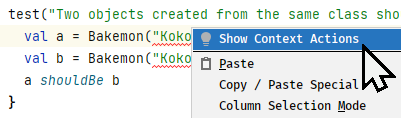
\includegraphics[width=0.5\textwidth]{img/oop/tdd/kotest_2/show_context_actions.png}
    \caption{Mostrar acciones de contexto}
    \label{fig:show-context-actions}
  \end{figure}

  \begin{figure}[ht!]
    \centering
    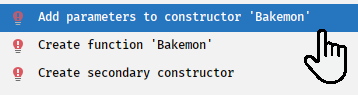
\includegraphics[width=0.5\textwidth]{img/oop/tdd/kotest_2/add_params_to_constructor.png}
    \caption{Agregar parámetros al constructor}
    \label{fig:add-params-to-constructor}
  \end{figure}

  \begin{figure}[ht!]
    \centering
    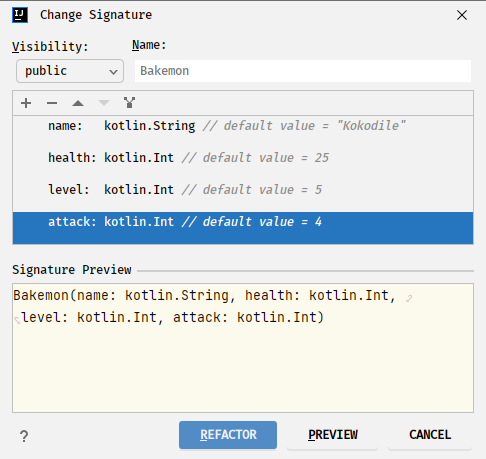
\includegraphics[width=0.5\textwidth]{img/oop/tdd/kotest_2/change_signature_of_constructor.png}
    \caption{Cambiar firma del constructor}
    \label{fig:change-signature-of-constructor}
  \end{figure}

  Perfecto, nuestro constructor ahora recibe parámetros.
  Lo siguiente que debemos hacer es guardar los parámetros en las propiedades correspondientes.
  Hagamos eso:

  \begin{kotlin}
    class Bakemon(name: String, health: Int, level: Int, attack: Int) {
      val name = name
      val health = health
      val level = level
      val attack = attack
      ...
    }
  \end{kotlin}
  
  Ahora, agreguemos los parámetros a los métodos \texttt{equals()}, \texttt{hashCode()} y
  \texttt{toString()}.

  \begin{kotlin}
    override fun toString(): String {
      return "Bakemon(name='$name', health=$health, level=$level, attack=$attack)"
    }

    override fun equals(other: Any?): Boolean {
      return when {
        this === other -> true
        other !is Bakemon -> false
        else -> name == other.name &&
            health == other.health &&
            level == other.level &&
            attack == other.attack
      }
    }

    override fun hashCode(): Int {
      return Objects.hash(Bakemon::class, name, health, level, attack)
    }
  \end{kotlin}

  Ahora sí, los tests deberían pasar.

  Como siempre, terminemos haciendo \textit{commit} de los cambios.

  \begin{powershell}
    git add .
    git commit -m "FEAT Adds name, health, level and attack to Bakemon"
  \end{powershell}